% =============================================================================
%  SANEN KINSEN HIROKU — Three Monkeys Gold Spring Secret Record
%  First English Translation
%
%  Source text attributed to: 牛田権三郎 (Ushida Gonzaburō)
%  Revised by: 鳴川猛之助 (Narukawa Takenosuke)
%  Manuscript: Kyoto University Main Library, Tanimura Collection (RB00012360)
%  License: Free with Attribution (二次利用自由・所蔵表示)
%
%  Edited and produced by Zach Booth
%  Translated with AI assistance (Claude, Anthropic)
%
%  Compiled with XeLaTeX
% =============================================================================

\documentclass[10pt, openany]{book}

\usepackage[
  papersize={6in,9in},
  margin=0.75in,
  inner=0.85in,
  outer=0.65in,
  top=0.8in,
  bottom=0.8in
]{geometry}

\usepackage{fontspec}
\setmainfont{Noto Serif}[
  BoldFont={Noto Serif Bold},
  ItalicFont={Noto Serif Italic},
  BoldItalicFont={Noto Serif Bold Italic},
]
\setsansfont{Noto Sans}
\newfontfamily\japanesefont{Noto Serif JP}[
  AutoFakeBold=2.5,
]
\newcommand{\jp}[1]{{\japanesefont #1}}

\usepackage{graphicx}
\usepackage{xcolor}
\usepackage{titlesec}
\usepackage{fancyhdr}
\usepackage{enumitem}
\usepackage{booktabs}
\usepackage{microtype}
\emergencystretch=1em  % Allow slightly looser line breaks to prevent overflow
\usepackage{hyperref}
\usepackage{float}
\usepackage{setspace}
\usepackage{lettrine}
\usepackage{parskip}
\usepackage{needspace}
\usepackage{mdframed}

\definecolor{chaptercolor}{HTML}{8B0000}
\definecolor{sectioncolor}{HTML}{333333}

\titleformat{\chapter}[display]
  {\normalfont\Large\bfseries\color{chaptercolor}}
  {\chaptertitlename\ \thechapter}{12pt}{\LARGE}
\titlespacing*{\chapter}{0pt}{-20pt}{20pt}

\titleformat{\section}
  {\needspace{4\baselineskip}\normalfont\large\bfseries\color{sectioncolor}}
  {\thesection}{1em}{}

\titleformat{\subsection}
  {\needspace{3\baselineskip}\normalfont\normalsize\bfseries\itshape\color{sectioncolor}}
  {\thesubsection}{1em}{}

% Prevent headings and first lines from being stranded at page bottom
\widowpenalties 3 10000 10000 150
\clubpenalties 3 10000 10000 150

\pagestyle{fancy}
\fancyhf{}
\fancyhead[LE]{\small\itshape Sanen Kinsen Hiroku}
\fancyhead[RO]{\small\itshape\leftmark}
\fancyfoot[CE,CO]{\small\thepage}
\renewcommand{\headrulewidth}{0.4pt}

% Footnotes use default \footnotesize (8pt at 10pt base)

% Translator's note footnote
\newcommand{\tn}[1]{\footnote{\textit{Translator's note:} #1}}

% Japanese term with romanization gloss
\newcommand{\jt}[2]{\jp{#1} (\textit{#2})}

% Editorial note: left bar, light background, smaller text
\definecolor{editorbg}{HTML}{F5F2EB}
\definecolor{editorbar}{HTML}{BBBBBB}
\newmdenv[
  topline=false,
  bottomline=false,
  rightline=false,
  linewidth=2pt,
  linecolor=editorbar,
  backgroundcolor=editorbg,
  innerleftmargin=10pt,
  innerrightmargin=10pt,
  innertopmargin=6pt,
  innerbottommargin=6pt,
  skipabove=8pt,
  skipbelow=8pt,
]{editorbox}
\newenvironment{editorialnote}{%
  \begin{editorbox}\small\textit{Editor's note:}\enspace}{\end{editorbox}}

\renewcommand{\chaptermark}[1]{\markboth{#1}{}}

\hypersetup{
  colorlinks=true,
  linkcolor=chaptercolor,
  urlcolor=blue!60!black,
  pdftitle={Sanen Kinsen Hiroku: Three Monkeys Gold Spring Secret Record},
  pdfauthor={Edited by Zach Booth; translated with AI assistance (Claude Opus 4.6, Anthropic)},
}

% Suppress hyperref warnings for CJK in PDF bookmarks
\pdfstringdefDisableCommands{\def\jp#1{}}
\pdfstringdefDisableCommands{\def\jt#1#2{#2}}

% =============================================================================
\begin{document}

% --- Half-title ---
\thispagestyle{empty}
\begin{center}
\vspace*{2.5in}
{\Large\itshape Sanen Kinsen Hiroku}\\[0.5em]
{\large Three Monkeys Gold Spring Secret Record}
\vfill
\end{center}
\newpage\thispagestyle{empty}\mbox{}\newpage

% --- Title page ---
\thispagestyle{empty}
\begin{center}
\vspace*{1in}
{\huge\bfseries\color{chaptercolor} \jp{三猿金泉秘録}}\\[1em]
{\LARGE\bfseries Sanen Kinsen Hiroku}\\[0.7em]
{\Large\itshape Three Monkeys Gold Spring\\Secret Record}\\[2em]
\rule{3in}{0.5pt}\\[1.5em]
{\large\itshape A Secret Record on the Art of\\Rice Market Speculation}\\[0.5em]
{\normalsize from the Edo Period of Japan}\\[2.5em]
{\normalsize Source text attributed to}\\[0.3em]
{\large \jp{牛田権三郎}}\\
{\normalsize Ushida Gonzabur\=o}\\[1.5em]
{\normalsize Revised and corrected by}\\[0.3em]
{\large \jp{鳴川猛之助}}\\
{\normalsize Narukawa Takenosuke}\\[2em]
\rule{3in}{0.5pt}\\[1.5em]
{\normalsize Edited and produced by Zach Booth}\\[0.3em]
{\small Translated with AI assistance}\\[3em]
\end{center}
\vfill
\newpage

% --- Copyright / attribution (page 1: provenance) ---
\thispagestyle{empty}
~\vfill

\begin{small}
\noindent\textbf{Source Manuscript}\\[0.3em]
\noindent\jp{校正三猿金泉秘録} (\textit{K\=osei Sanen Kinsen Hiroku})\\
Record ID: RB00012360\\
Tanimura Collection (\jp{谷村文庫})\\
Main Library, Kyoto University (\jp{京都大学附属図書館})\\[0.5em]
Date: 20th day, 5th month, Kaei 4 (\jp{嘉永四年五月廿日}; 1851).
Sexagenary year: \jp{辛亥} (\textit{kanoto-i})\\
Publisher: K\=omond\=o (\jp{好問堂蔵版})\\
Location: Igarashi-tsu (\jp{五十嵐津})\\
Manuscript type: Copy (\jp{写}) of the K\=omond\=o edition\\
Subtitle: \jp{温故知新活法窮理} (\textit{Onko chishin kapp\=o
k\=uri})---``Investigating principles through the living method of
studying the old to know the new''\\
Supplement: \jp{天問秋作見積之圖 補附}---``With appended diagrams of
autumn harvest estimation by heavenly inquiry''\\[1em]

\noindent\textbf{Digital Images}\\[0.3em]
\noindent Kyoto University Rare Materials Digital Archive\\
\url{https://rmda.kulib.kyoto-u.ac.jp/item/rb00012360}\\[0.5em]
Free License with Attribution (\jp{二次利用自由（所蔵表示）})\\
Reuse policy: \url{https://rmda.kulib.kyoto-u.ac.jp/reuse}\\[1em]

\noindent\textbf{Attribution}\\[0.3em]
\noindent All manuscript images courtesy of the Main Library, Kyoto University.\\
\jp{所蔵：京都大学附属図書館}\\[1em]

\noindent\textbf{Open Source}\\[0.3em]
\noindent The complete methodology---including manuscript scans,
character-by-character transcription, working translation files, and
\LaTeX{} source---is available at
\url{https://github.com/groverburger/sanen-kinsen-hiroku}.
\end{small}
\newpage

% --- Copyright / attribution (page 2: edition info) ---
\thispagestyle{empty}
~\vfill

\begin{small}
\noindent English translation copyright \textcopyright{} 2026 Zach Booth.
All rights reserved. The \LaTeX{} source and methodology are released
under CC BY-NC-SA 4.0.\\[0.5em]
ISBN 979-8-254-10079-9\\[1em]

\noindent\textbf{About This Edition}\\[0.3em]
\noindent This is the first English translation of the \textit{Sanen Kinsen
Hiroku}. The manuscript was sourced and the translation project directed
by Zach Booth. The translation from classical Japanese was produced with
AI assistance (Claude Opus 4.6, Anthropic), which read the original
manuscript page images directly using multimodal capabilities. The
original text is written in \textit{kobun} (classical Japanese) with
\textit{kanbun kundoku} reading marks in cursive script
(\textit{kuzushiji}) on aged paper.\\[0.5em]
\noindent\textbf{On Confidence.} The translation was produced in two
stages: first a character-by-character transcription of the Japanese
with confidence levels, then an English translation from that
transcription. Section headers, diagram labels, numerical tables, and
structured lists (such as the sexagenary year cycles) are generally
legible and reliably translated. Connecting prose between these anchors
varies widely in legibility: some passages are clearly readable, while
others---particularly in dense cursive sections---are partially or
largely illegible at the available scan resolution. Where the
manuscript is difficult to read, the translation is marked as
interpretive. Passages flagged ``\textit{interpretive}'' represent our
best reconstruction of the text's meaning from partial readings and
contextual clues; they should not be cited as the author's exact
words.\\[1em]

\noindent\textbf{How to Read This Translation}\\[0.3em]
\noindent The body text of this book is a direct translation of the source
manuscript. The chapter and section headings are editorial, added for
navigation. Footnotes marked ``\textit{Translator's note}'' provide
historical context, definitions, and comparative observations. Rare
indented passages marked ``\textit{Editor's note}'' provide brief
editorial bridges where the manuscript's structure requires explanation. Chapter lengths vary because
the translation follows the manuscript's own proportions---some topics
receive extensive treatment in the source, others only a line or two.
Passages marked ``\textit{Interpretive}'' are
reconstructions from partially legible manuscript sections; all other
body text is a direct translation of the source.\\[0.5em]
\noindent\textbf{Structure of the Text.}
Chapters 1--2 establish the cosmological framework and seasonal trading
rules. Chapters 3--4 present the mechanics of staged entry and the
sixty-year weather cycle. Chapters 5--8 build the decision
framework: market forces, the four virtues, the Middle Star
mean-reversion system, and the Seven Fortunes. Chapter~9 synthesizes
everything in the Grand Diagram. Chapters 10--11 close with
sentiment-reading and final teachings.
\end{small}
\newpage

% =============================================================================
\thispagestyle{empty}
\tableofcontents
\newpage

% =============================================================================
\chapter*{Translator's Introduction}
\addcontentsline{toc}{chapter}{Translator's Introduction}
\markboth{Translator's Introduction}{}

The \textit{Sanen Kinsen Hiroku} (\jp{三猿金泉秘録}), or ``Three Monkeys
Gold Spring Secret Record,'' is one of the most celebrated texts in the
history of Japanese market speculation.\tn{The manuscript is dated
\jp{嘉永四年五月廿日} (1851) and identifies itself as a copy of the
K\=omond\=o (\jp{好問堂}) edition, published at Igarashi-tsu
(\jp{五十嵐津}). The text references the Tenmei era (1781--1789)
extensively for its price data.}

\begin{sloppypar}
The title alludes to the proverb of the three
monkeys---``see no evil, hear no evil, speak no evil''
(\jp{見ざる、聞かざる、言わざる})---reinterpreted
as a warning to the trader: do not be swayed by what you \textit{see} others
doing, what you \textit{hear} as rumor, or what you \textit{say} in haste.
Instead, observe the deeper patterns.
\end{sloppypar}

\section*{Authorship and the Edo Rice Market}

The manuscript names its author as Ushida Gonzabur\=o (\jp{牛田権三郎}),
an Osaka D\=ojima trader from Ise province who wrote under the pen name
Jiunsai (\jp{慈雲斎}). The text was composed around 1755 and later
revised and corrected by Narukawa Takenosuke (\jp{鳴川猛之助}). It
belongs to a genre of ``secret market transmission texts''
(\jp{相場秘伝書}, \textit{s\=oba hidensho}) that circulated among
Edo-period trading houses.\tn{The inner title page of the manuscript
appears to bear a small label that may read \jp{三猿軍書選}
(\textit{Sanen gunsho sen}, ``Selection from the Three Monkeys
Military/Strategy Books''), though the label is partially obscured and
this reading is uncertain.}

During the Tokugawa period (1603--1868), rice was the basis of the economy.
The D\=ojima Rice Exchange (\jp{堂島米会所}) in Osaka functioned as a
sophisticated futures market where ``book rice'' (\jp{帳合米}) was traded
as forward contracts.\tn{The D\=ojima Rice Exchange was established in 1697
as a spot market. Organized futures trading (\jp{帳合米}) was formally
authorized by the shogunate in 1730, making it one of the world's first
organized futures markets.}

\section*{A Note on Attribution}

English-language sources almost universally attribute this text to Honma
Munehisa (\jp{本間宗久}) of Sakata, often under the title ``The Fountain
of Gold---The Three Monkey Record of Money.'' This attribution is
incorrect.

The manuscript names its author as Ushida Gonzabur\=o and its editor as
Narukawa Takenosuke---as do the National Diet Library catalog, the CiNii
bibliographic record, and every Japanese-language reference work that
discusses it. In Japanese scholarship, this is not controversial:
the NDL, CiNii, Kyoto University's digital archive, and sources from
Honma's own hometown (the Shonai Securities company of Sakata) all
attribute the \textit{Sanen Kinsen Hiroku} to Ushida.

Honma Munehisa was a real historical figure---a Sakata trader who was
expelled from his own family for speculating with company capital and who
became legendary in his own right. Texts were later attributed to him
(the \textit{S\=oky\=u-\=o Hiroku} and \textit{S\=oba Sanmai-den}),
though no Edo-period originals of these survive; Japanese scholars suspect
they were compiled in the Meiji era. Honma's texts have entirely different
titles and contents from Ushida's.

The confusion appears to have entered English through Steve Nison's
influential \textit{Japanese Candlestick Charting Techniques} (1991),
a book that did enormous service in introducing Japanese technical
analysis to Western traders. In synthesizing a large body of
Japanese-language material for an English-speaking audience, Nison
consolidated several distinct figures and texts into a single
narrative---an understandable simplification given the complexity of the
source tradition. Nison himself corrected the record in
\textit{Beyond Candlesticks} (1994, p.\,14), writing that his research
indicated Honma ``likely did not use candlestick charts.'' But the first
book reached millions of readers, and the broader conflation of names
and titles took on a life of its own.

In the decades since, English sources have merged Ushida's title with
Honma's name, creating a phantom text: ``The Fountain of Gold'' (\jp{金泉})
and ``Three Monkeys'' (\jp{三猿}) are both from Ushida's title; the Honma
texts have completely different names. Two English-language books have been
published under variations of this text's title. Neither translates it.
Both render a separate body of trading maxims from the Honma/Sakata
tradition---a related but distinct lineage---while putting Ushida's title
on the cover.

What follows is, to my knowledge, the first English translation of the
actual \textit{Sanen Kinsen Hiroku}, made directly from the 1851
manuscript held at Kyoto University.

\vspace{1em}
\begin{flushright}
\textit{---Zach Booth}
\end{flushright}

% =============================================================================
\chapter{Preface: The Cosmology\\ of the Market}

\begin{center}
\jp{三猿金泉録序}\\[0.3em]
\textit{Preface to the Three Monkeys Gold Spring Record}
\end{center}

\vspace{1em}

\lettrine[lines=2]{T}{he Supreme Ultimate}\tn{\jp{太極} (\textit{taikyoku}).
The foundational concept of Neo-Confucian cosmology. The opening echoes
Zhou Dunyi's \textit{Taijitu shuo} (Explanation of the Diagram of the
Supreme Ultimate, mid-11th century), grounding market theory in the highest
philosophical authority.}
moves and gives birth to Yang; when still, it gives birth to Yin.
The principle of one stillness and one movement---Heaven and Earth rise and
fall according to this logic. Movement reaches its extreme and becomes
stillness; stillness reaches its extreme and becomes movement again.
Movement and stillness are the root of one another.

This is the principle by which strong qi\tn{\jp{強気} (\textit{tsuyoki}),
literally ``strong spirit''---bullish sentiment. Its opposite, \jp{弱気}
(\textit{yowaki}), ``weak spirit,'' is bearish sentiment.} and weak qi
alternate.

When this principle is applied to all things, there is nothing it does not
encompass. When applied to rice, the qi of people---whether strong or
weak---is contained within this principle. Those who combine this
understanding with close observation of the market will find it reasonable.
In years of good harvests and times of fine weather, one should compare and
examine the rice markets.

This is the principle that transcends mere natural disposition.

In recent years, new rice arriving in the ninth and tenth months has been
declining in price. When rice falls, strong buying emerges---this is the
buying pattern. Conversely, when rice has been rising for some months,
selling pressure appears at the ceiling.\tn{The manuscript's cursive
becomes significantly denser in this passage. The general sense---that
buying follows price declines and selling follows rises---is clear from
the legible characters, but individual phrases are uncertain.}

Within a cycle of favorable and adverse conditions spanning twelve or
thirteen years, the secret records of the house---the family tradition
spanning thirty generations---are secretly stored. This is the family
tradition of Ushida Gonzabur\=o.\tn{The numbers ``twelve or thirteen''
and ``thirty'' are legible. The intervening text is heavily damaged
cursive; the passage may reference a capital figure (possibly
\jp{千五百}, 1,500) but the reading is too uncertain to render with
confidence.}

% =============================================================================
\chapter{Favorable and Adverse Conditions;\\ The Articles of Trading}

\section{Favorable and Adverse Conditions}

\begin{center}
\jp{順来・逢来} --- \textit{Junrai and Airai}
\end{center}

\vspace{0.5em}

\begin{editorialnote}
Two units recur throughout the text that follows.
\jt{両}{ry\=o}: the standard gold coin of the Edo period, used here as
the unit of trading capital. \jt{俵}{tawara}: a bale of rice, the
standard unit of measure for rice trading and price quotation. Gold and
rice---ry\=o and tawara---are the two axes of every calculation in this
text.
\end{editorialnote}

The market moves in great cycles of favorable conditions
(\jt{順来}{junrai}) and adverse conditions (\jt{逢来}{airai}). Within a
period of roughly twelve to thirteen years, favorable conditions persist for
approximately ten years, and adverse conditions for three.\tn{This roughly
10:3 ratio of bull-to-bear years anticipates modern observations about
market asymmetry---that markets spend more time rising than falling, but
that the falls are sharper.}

During favorable years, rice is generally at high levels. When old rice
(\jt{古米}{komai})\tn{Rice from previous harvests, as opposed to
\jp{新米} (\textit{shinmai}), newly harvested rice. Old rice was traded as
a distinct commodity.} is in a year of abundance, it will be cheap. Buy in
the fourth month. By mid-sixth month, prices will be high---this is where
one sells. In autumn, buy again around the seventh month. Toward year-end,
the price of old rice will rise, and one should sell again.\tn{The month
references (fourth, sixth, seventh) are partially legible in the
manuscript. The surrounding trading instructions are interpretive,
reconstructed from these anchor points and the section's overall theme.}

This is the fundamental pattern of favorable years.

In adverse years, the cheap period for old rice falls around the fourth
through sixth months. In autumn, one should buy, and by year-end the rice
price climbs.

\needspace{14\baselineskip}
A song (\jp{歌}, \textit{uta}) on favorable conditions for the four
seasons, and the estimation of highs and lows:\tn{The source text
identifies this passage as an \textit{uta}---a verse or mnemonic poem,
a common device in Edo-period instructional texts for making key
principles memorable. The \jp{歌} label and the four-seasons/high-low
theme are legible; the specific verse text below is an interpretive
reconstruction from partially readable cursive.}

\begin{verse}
\textit{[Interpretive.]}\\
In a year of favorable conditions,\\
the autumn harvest is plentiful;\\
the highs and lows can be estimated\\
across four seasons.\\[0.5em]
In spring, from around the fourth month onward,\\
buy at the fifth-month level;\\
by the end of the year,\\
the high price will come.
\end{verse}

In favorable periods, the rice market's sentiment (\jt{人気}{jinki})\tn{%
Literally ``people-qi''---the collective mood of market participants.} for
each month can be read directly. The fifth-month and year-end levels become
the reference points. In a year of great flood, the rice market reacts
through the twelfth month.

\section{The Fifteen Articles of Trading}

\begin{center}
\jp{十五ヶ条 禁物場} --- \textit{J\=ugo Kaj\=o, Kinmotsu-ba}\\
\textit{Fifteen Articles: Forbidden Things of the Marketplace}
\end{center}

\vspace{0.5em}

\tn{The section heading names fifteen articles, but the manuscript presents
them as flowing prose punctuated by cautionary markers (\jp{禁判},
\textit{kinban}, literally ``forbidden judgment'') rather than as a numbered
list. Approximately six to eight distinct \jp{禁判} markers are legible in
the cursive script. Whether the remaining articles were lost in
transmission, are embedded in the prose without explicit markers, or whether
``fifteen'' is a conventional number for such collections is unclear from
this manuscript. What follows is a faithful translation of the legible
text.}

\begin{editorialnote}
The manuscript contains six to eight \jp{禁判} (cautionary) markers with
surrounding prose in dense cursive. The markers themselves are legible;
the text between them is only partially readable. What follows is an
interpretive reconstruction: the general themes are consistent with the
legible fragments (terms like \jp{世の人}, \jp{売買}, \jp{強弱の気},
\jp{新米}, \jp{秋} are identifiable), but the specific phrasing should
not be taken as the author's exact words.
\end{editorialnote}

\textit{[Interpretive.]}
Within the market, one must read the sentiment of the crowd---whether people
are inclined to buy or sell---and not act rashly.

\jp{禁判}: The large trader may think that because he has capital, he can
afford to hold a losing position. This is a grave error. Even with great
capital, if one buys recklessly and the market moves against him, the losses
compound. Conversely, a trader of modest means who reads the market well
and trades with discipline can accumulate wealth steadily.

\jp{禁判}: The decision to buy or sell should not be made lightly. One
should observe for several days.

\jp{禁判}: Do not follow the crowd blindly. When all are buying, consider
selling; when all are selling, consider buying. The profit lies in going
against common sentiment, yet one must have sound reason for doing
so.\tn{The contrarian principle (\jp{世の人}---``the people of the
world''---and \jp{売}/\jp{買} are among the legible characters in this
passage) predates the Western maxim ``buy when there is blood in the
streets'' (apocryphally attributed to Baron Rothschild).}

\jp{禁判}: Those who deal in large quantities and those with small capital
must both observe these rules equally.

\jp{禁判}: In the autumn months, when new rice enters the market and the
old rice price adjusts, one must read the market carefully.

\jp{禁判}: When the people of the world (\jp{世の人}) are of one mind
regarding the market, the strong and weak sentiments must be weighed.

\begin{editorialnote}
Several further \jp{禁判} markers are present in the manuscript but the
surrounding cursive text is too damaged or faded to translate with
confidence.
\end{editorialnote}

\section{The Thirty-Eight Provisions for Seasonal Trading}

\begin{center}
\jp{三十八ヶ条 商内} --- \textit{Sanj\=uhachi Kaj\=o, Sh\=onai}\\
\textit{Thirty-Eight Provisions for Trading}
\end{center}

\vspace{0.5em}

\tn{As with the Fifteen Articles, the heading names thirty-eight provisions,
but the manuscript presents them as continuous prose about seasonal trading
rather than a numbered enumeration. The provisions are woven into the
narrative of monthly and seasonal patterns. Whether a fully enumerated
version existed in another recension of the text is unknown.}

In a year of adverse conditions (\jp{逢来}), from around the fifth month
onward, summer rice drops and autumn months see further decline. Autumn
months are for buying; favorable months are for the pattern of waiting.

In a year of good harvest (\jt{上作}{j\=osaku}), rice is abundant and
prices are depressed.\tn{\jp{上作}/\jp{中作}/\jp{下作} refer to harvest
quality grades---good, average, and poor.
\jp{上作} (literally ``upper crop'') is an abundant harvest; \jp{下作}
(``lower crop'') is a poor one.} In an average harvest
(\jt{中作}{ch\=usaku}), prices fall between the extremes. In a poor
harvest (\jt{下作}{gesaku}), rice is scarce and prices rise.

In a year of favorable conditions, from spring onward: if the harvest is
expected to be plentiful, summer rice will be cheap. Buy in the third or
fourth month at the low, and sell by the middle of the sixth month when the
price has risen.

In autumn, buy again at the harvest-month low. By year-end, old rice prices
climb, and this is where one takes profit.

In an adverse year, the pattern reverses. From the fifth month, prices
decline through summer. The autumn months are the buying months. By the
year-end, prices recover.

For the months from the tenth onward, consider the first ten days of each
month. The market's movement can be read within each four-to-five month
period.

In the fifth month, in a year of poor harvest, the rice situation becomes
tight; one should buy at the lower level. But in a strong-yield period of
four years, the rice pattern reverses.

The sentiment of the rice market (\jp{米來人気筋}) can be read directly from
the monthly price action. The favorable-condition months and the
adverse-condition months each have their own character. The trader who reads
them alongside the harvest forecast can establish the full year's plan.

When weak qi pervades the world and things seem to continue weakening, yet
the rice price is at a level that appears flat---this is the year of rice
buying.\tn{The last two sentences of this section in previous editions
(``The flat price amid universal pessimism\ldots'') were editorial
additions without manuscript support and have been removed.}

% =============================================================================
\chapter{The Record of Patterns\\ and Staged Entry}

\section{Record of Spike Patterns}

\begin{center}
\jp{穂足の録}\tn{Literally ``grain-spike form''---\jp{穂}
(ear of rice) plus \jp{足} (form/trace). In modern Japanese trading,
\jp{足} is the standard suffix for price-chart types:
\jp{ローソク足} (candlestick), \jp{日足} (daily bar), \jp{棒足}
(bar chart), etc. Whether \jp{穂足} is an early instance of this
convention is uncertain, but the shared suffix and agricultural
metaphor are suggestive.} --- \textit{Hosoku no Roku}
\end{center}

\textit{[Interpretive.]}
When buying and holding, one must consider the fortune (\jt{運}{un}) and the
momentum (\jt{気}{ki}). The seasonal movements and patterns across two
hundred days must be compared.\tn{The terms \jp{運} and \jp{気} and the
figure \jp{二百日} are tentatively legible. The remainder of this section
is in dense cursive rated LOW confidence; the prose below is
reconstructed from fragmentary readings and the section's context.}

One should not be impatient: observe for two or three days, then when the
rice begins to move, buy. Those who buy impulsively and hold stubbornly will
fail.

\section{The Scaling Diagrams}

\begin{center}
\jp{萬光商内之圖}\\
\textit{Bank\=o Sh\=onai no Zu --- Diagram of Ten-Thousand-Light Trading}
\end{center}

\begin{figure}[H]
\centering
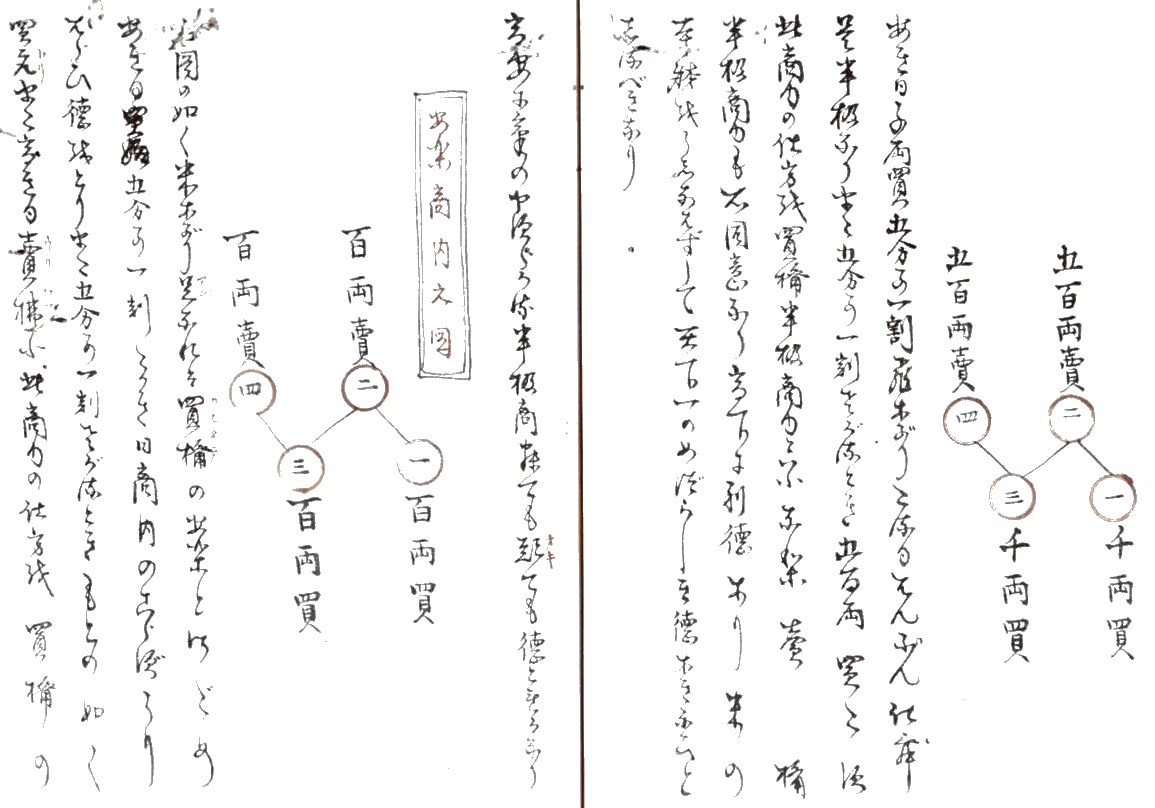
\includegraphics[width=\textwidth]{diagrams/fig1_tree_positions.png}
\caption[Position-scaling diagrams]{Position-scaling diagrams from the original manuscript.
Right page: building from a base purchase (\jp{千十両買})\tn{The
cartouche reads \jp{千十両買}, which could be parsed as ``1,000+ ry\=o
buy'' or ``1,010 ry\=o buy.'' The transcription flags this as
ambiguous; we follow the more natural reading of ``1,000-ry\=o base
purchase.''}
through four stages to a 500-ry\=o position (\jp{五百両買}). Left page:
the 100-ry\=o sell diagram (\jp{百両売}) and a second scaling diagram
under the boxed label \jp{萬光商内之圖}.
\textit{Image: Kyoto University Main Library.}}
\label{fig:tree1}
\end{figure}

The diagrams show a method of building and unwinding positions through
numbered stages. Starting from a base purchase, the position is built
through four stages marked \jp{壱}, \jp{弐}, \jp{参}, \jp{四}.\tn{The
stage markers (\jp{壱}--\jp{四}) are clearly legible in red ink in the
diagrams. The prose describing what each stage represents is interpretive;
the manuscript text surrounding the diagrams is in dense cursive that
resists character-level reading.}

\section{The Turnover Method}

\begin{figure}[H]
\centering
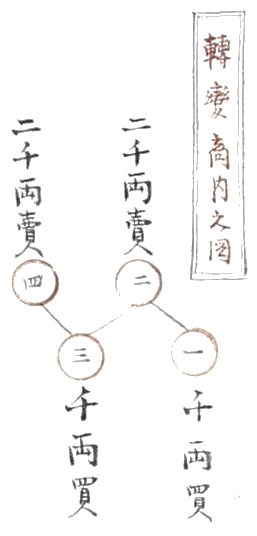
\includegraphics[width=0.45\textwidth]{diagrams/fig2_tree_scaling.png}
\caption[The turnover diagram]{Detail from the scaling diagrams showing the
turnover method. The diagram labels \jp{百両買} (100-ry\=o buy, bottom)
and \jp{百両賣} (100-ry\=o sell, top) are legible, with four stage
markers (\jp{壱}--\jp{四}) in red ink. \textit{Image: Kyoto University
Main Library.}}
\label{fig:tree2}
\end{figure}
\textit{[Interpretive.]}
When buying positions reach their target, begin to build selling positions
simultaneously---this is the turnover method (\jt{転換の法}{tenkan no
h\=o}). For every 1,000 ry\=o in buying positions, prepare to sell 2,000
ry\=o worth.\tn{The term \jp{転換の法} and the 1,000/2,000 ratio are
supported by partially legible text on the left page of page~13. The
extended prose that follows is interpretive, reconstructed from
fragments and the diagram's structure.}

When traders see profits growing, they become greedy and wish to hold
longer. When they see losses, they become fearful and wish to sell at once.
Both impulses are the enemy of profit.

% =============================================================================
\chapter{The Sixty-Year Cycle: Weather, Tides, and Harvest}

\begin{center}
\jp{暴風 運気豊凶之録}\\
\textit{Record of Storms, Fortune-Qi, and Abundance or Famine}
\end{center}

\vspace{0.5em}

A twelve-year sub-cycle governs the alternation of fortune and misfortune in
harvests. Two hundred and thirty years of records were consulted, tracking
patterns of weather and their correlation with the sexagenary cycle
(\jt{干支}{kanshi}).

\begin{editorialnote}
The years in this chapter are named using the sexagenary cycle, which
pairs one of ten Heavenly Stems
(\jp{甲乙丙丁戊己庚辛壬癸}) with one of twelve Earthly Branches
(\jp{子丑寅卯辰巳午未申酉戌亥}). The
combinations produce a sixty-year cycle before repeating. Each year has
a unique two-character name: \jp{甲子} (\textit{kinoe-ne}) is year~1,
\jp{乙丑} (\textit{kinoto-ushi}) is year~2, and so on through all
sixty. As a rough guide to Western dates: \jp{甲子} corresponds to
1744, 1804, and 1864; each designation recurs every sixty years.
\end{editorialnote}

\section{Violent Storms}

In certain years, violent storms and market surges are more frequent:
\jp{甲子}~(1), \jp{丁卯}~(4), \jp{丁未}~(44), \jp{甲戌}~(11),
\jp{甲申}~(21), \jp{辛卯}~(28), \jp{甲午}~(31).\tn{The numbers in
parentheses indicate the year's position within the sixty-year cycle.}
In these years, rice markets experience extreme volatility; prices may
surge two or three times within a single season.

\section{Floods}

Years containing \jp{己} (\textit{tsuchinoto}) in their stem are associated
with water disasters: \jp{己巳}~(6), \jp{己卯}~(16), \jp{己丑}~(26),
\jp{己亥}~(36),
\jp{己酉}~(46), \jp{己未}~(56). These bring three-year periods of
disruption.

\section{Frost and Cold}

Unusual cold damages crops: \jp{己巳}~(6), \jp{己亥}~(36),
\jp{己未}~(56). These trigger three-year adverse periods. Rice prices
rise sharply.

\section{Bountiful Harvest Years}

Years of bountiful harvest (\jt{豊作}{h\=osaku}) were tracked across
twenty-eight years of records and correlated with the sexagenary cycle. In
autumn months, yields were logged, producing a predictive framework
spanning the full sixty-year cycle.

\section{The Plum Rains}

The onset of the plum rain season (\jt{梅立}{tsuyudachi})\tn{%
The manuscript uses \jp{梅立} (\textit{tsuyudachi}, ``plum rains onset'')
rather than the more common modern term \jp{梅雨} (\textit{tsuyu}).} follows an
approximately eight-year sub-cycle. Early plum rains generally indicate good
harvests. Late plum rains may indicate drought followed by flooding.

Associated years: \jp{丙寅}~(3), \jp{丙子}~(13), \jp{庚辰}~(17),
\jp{庚寅}~(27), \jp{壬午}~(19), \jp{壬辰}~(29), \jp{丙申}~(33),
\jp{丙午}~(43).

\section{Tides}

\begin{center}
\jp{大潮小潮之差} --- \textit{The Difference Between Spring and Neap Tides}
\end{center}

\vspace{0.5em}

\textit{[Interpretive.]}
The patterns of spring tides (\jp{大潮}) and neap tides (\jp{小潮})
bear on weather prediction.\tn{The section header \jp{大潮小潮之差} is
clearly legible. The prose beneath it is in dense cursive and largely
illegible at the available scan resolution; claimed furigana readings
for these terms cannot be confirmed. The interpretive text here
reflects the section's apparent theme.} In years of great tidal
difference, storms are more likely.

\section{Wind}

Wind direction and timing follow their own cycles: \jp{戊申}~(45),
\jp{己卯}~(16), \jp{丙辰}~(53), \jp{丁巳}~(54), \jp{庚申}~(57). In
years of strong autumn wind, harvest
damage increases. The period between the seventh and ninth months is
critical.

A ten-year or fifteen-year span governs the wind's major directional shifts.
Across one hundred years of observation, these cycles hold with reasonable
reliability---roughly one year of error in every ten.

% =============================================================================
\chapter{The Eight Poles, Celestial Signs, and the Six Observations}

\section{The Eight Poles}

\begin{center}
\jp{八極 三千目} --- \textit{Eight Poles, Three Thousand Points}
\end{center}

\vspace{0.5em}

The categories of market force: Yang (\jp{陽})---the bullish, rising force.
Yin (\jp{陰})---the bearish, falling force. The Supreme Ultimate
(\jp{太極})---equilibrium. Yin convergence (\jp{陰合})---multiple bearish
factors aligning at once.

\subsection{The Force of One-Nine (\jp{一旅将壱九之勢})}

\textit{[Interpretive.]}
When ten thousand people are all of one mind---all buying or all
selling---the reversal is near. A thousand people of the same opinion is a
strong signal. Ten thousand unanimous is an extreme.\tn{The header
\jp{一旅将壱九之勢} is legible. The terms \jp{万人} and \jp{千人} are
tentatively identifiable in the surrounding cursive; the connecting prose
is interpretive.}

\section{Celestial Anomalies}

\begin{center}
\jp{天怪} --- \textit{Tenkai}
\end{center}

\vspace{0.5em}

\textit{[Interpretive.]}
When extraordinary signs appear---unusual weather, disruptions to the normal
seasonal flow---first determine whether these are temporary or lasting in
their effect.\tn{The header \jp{天怪} is clearly legible. The prose
beneath it is in dense cursive; this rendering reflects the section's
apparent theme but cannot be confirmed character by character.}

\section{The Six Observations}

\begin{center}
\jp{六初覚} --- \textit{Roku Shokaku}
\end{center}

\vspace{0.5em}

When watching the rice market, first observe these six
things:\tn{These six observations form a structured checklist---essentially
a pre-trade evaluation framework.}

\begin{enumerate}[leftmargin=2em]
\item The 20\% level (\jt{二割}{ni-wari}).
\item The 30\% level (\jt{三割}{san-wari}).
\item Within the high range (\jt{高の内}{taka no uchi}).
\item Sideways movement (\jt{横の平}{yoko no hira}).
\item People's sentiment (\jt{人の気}{hito no ki}).
\item The grand trend (\jt{大勢}{taisei}).
\end{enumerate}

\tn{All six Japanese terms are clearly legible with furigana in the
manuscript. The prose that follows is interpretive, reconstructed from
partially legible cursive that includes the characters \jp{山} (mountain)
and \jp{千人} (a thousand people).}

\textit{[Interpretive.]}
These six observations determine all trading. When wishing to buy, first
check whether the price has already risen 20--30\% from its base.

All buying and selling should be done proportionally. When buying, think of
mountains---rice is like mountains and water. The great mountain does not
rise in a day.

When a thousand people are of one mind regarding the market, and a single
trader perceives something different, he must weigh his own observation
against the crowd's.

% =============================================================================
\chapter{The Four Virtues of the Trader}

\section{Benevolence (\jp{仁}, \textit{Jin})}

Buy once, and it returns to its original level.
Wait.\tn{The source text names four virtues: Benevolence (\jp{仁}),
Wisdom (\jp{智}), Courage (\jp{勇}), and Discipline (\jp{節}). The
traditional Confucian system names five constant virtues (\jp{五常}),
the fifth being Trustworthiness (\jp{信}, \textit{shin}). Whether the
fifth was omitted deliberately or lost in transmission is unknown from
this manuscript.}\tn{The manuscript heading for this section reads
\jp{仁 — 壱首・壱百五拾目} (\textit{Jin --- Isshu, hyaku goj\=u me}),
meaning ``Benevolence---First article; the 150th item.'' This reference
to 150 is unexplained and may indicate the text draws from a larger
collection of trading rules.}

\textit{[Interpretive.]}
When one buys and the price returns to the purchase level, do not panic
and sell at cost.\tn{The opening line \jp{壱買段せ、其まゝ本へもどる} is
legible; the prose that follows is in denser cursive with the figure
\jp{三年} (three years) partially legible. The remaining phrasing is
interpretive.}

If after buying, the price falls and then recovers, this pattern---repeated
over three years---teaches the trader to endure.

\subsection{On Upper, Middle, and Lower Positions}

At the upper level (\jt{上位}{j\=oi}), rice has risen strongly and is at
the top of its range. One should be selling, not buying. At the middle
level (\jt{中位}{ch\=ui}), rice is at its ordinary seasonal level; wait
and observe. At the lower level (\jt{下位}{gei}), rice has fallen to the
bottom of its range. This is where buying begins.

When the price has been at a low level for three hundred days or more, and a
rise begins, and then the price returns and falls again to a new low---this
is the final bottom. Buy here.

\section{Wisdom (\jp{智}, \textit{Chi})}

The manuscript heading reads \jp{智 十首} (``Wisdom---Ten Principles'').
The body text beneath this heading is in dense cursive that resists
character-level reading; its specific content cannot be reliably
translated.\tn{The header \jp{智 十首} is clearly legible. The
surrounding prose is rated LOW confidence in the transcription.}

\subsection{The Standard of Calm Profit (\jp{平楽定式})}

\textit{[Interpretive.]}
Buying is done at a set price level; one then holds until the target
selling month.\tn{The header \jp{平楽定式} is legible. The body text is
in dense cursive rated LOW confidence; this rendering is interpretive.}

\subsection{Regional Market Timing}

\textit{[Interpretive.]}
The relationship between different regional markets---D\=ojima, Bakan, and
others---creates timing advantages. Information flows between them with
delay.\tn{References to \jp{大坂堂島} and \jp{馬関} are tentatively
identifiable in the cursive. The connecting prose is reconstructed from
these anchor terms.}

\section{Courage (\jp{勇}, \textit{Y\=u})}

The manuscript's treatment of this virtue is very brief and in dense
cursive. The heading \jp{勇} is legible; the body text cannot be reliably
translated.

\section{Discipline (\jp{節}, \textit{Setsu})}

\textit{[Interpretive.]}
The cautious man holds \jt{陸金}{rikukin}\tn{\jp{陸金} literally ``land
gold''---stable reserves kept out of the market. This passage appears in
the manuscript within the ``Following Gold'' (\jp{随金}) section
(page~27); it is placed here under ``Discipline'' for thematic coherence.
The heading \jp{節} is legible; the body text is partially legible, with
\jp{陸金}, \jp{二十俵}, and \jp{五} tentatively identifiable.}
of twenty tawara and trades with five.

% =============================================================================
\chapter{The Three Levels and the Middle Star}

The total yields (\jp{諸高}) of all rice-producing domains, combined:
28,548 \textit{ch\=o},\tn{\jp{町} (\textit{ch\=o}), a unit of
land area approximately equal to 2.45 acres or 1 hectare. The figure
represents the total productive rice land across all domains, used to
calculate the autumn harvest estimate.} comprising 9,484,815
\textit{tawara} in autumn harvest estimates.

\begin{center}
\jp{世の中 三段之圖}\\
\textit{Diagram of the Three Levels of the World}
\end{center}

\begin{figure}[p]
\centering
\vspace*{\fill}
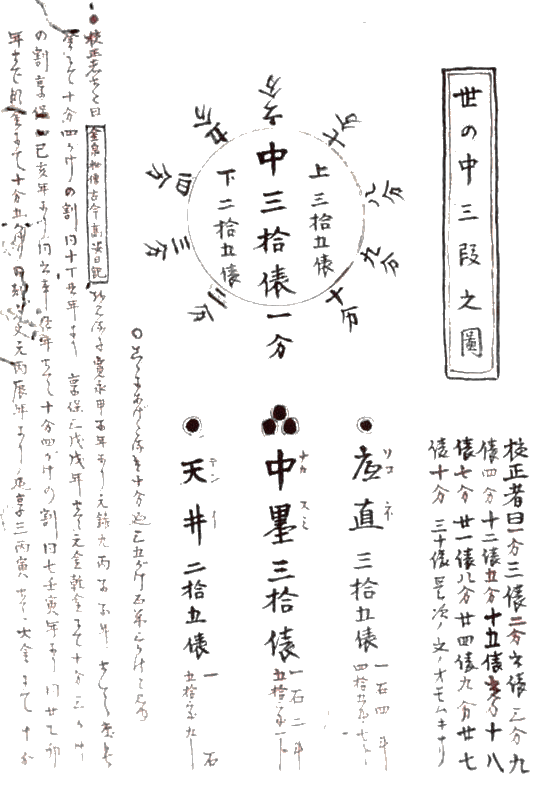
\includegraphics[width=0.75\textwidth]{diagrams/diagram_three_levels.png}
\caption[The Three Levels Diagram]{The Three Levels Diagram (\jp{世の中三段之圖}). The circle is
divided into Upper (\jp{上}, 35 tawara supply), Middle (\jp{中}, 30
tawara), and Lower (\jp{下}, 25 tawara supply). Below: the Ceiling
(\jp{天井}, price peak at lowest supply), Floor (\jp{底直}, price
trough at highest supply), and Middle Star (\jp{中星}, equilibrium)
reference points with their associated calculation tables.
\textit{Image: Kyoto University Main Library.}}
\label{fig:threelevels}
\vspace*{\fill}
\end{figure}

\section{The Three Levels}

The rice market at any moment exists within one of three supply
ranges.\tn{The tawara figures here measure rice \textit{supply}, not
price. The relationship to price is inverse: when supply is high (35
tawara), rice is abundant and prices are low; when supply is low (25
tawara), rice is scarce and prices are high. Thus \jp{天井}
(\textit{tenj\=o}, price ceiling---the highest price point) corresponds
to the \textit{lowest} supply level (25 tawara), and \jp{底直}
(\textit{soko-ne}, price floor---the lowest price point) corresponds to
the \textit{highest} supply level (35 tawara).} The upper supply level
(\jp{上}): approximately 35 tawara---rice is abundant, prices are at
their floor (\jp{底直}); this is where buying is indicated. The middle
level (\jp{中}): approximately 30 tawara, 1 bu---equilibrium, where one
observes and waits. The lower supply level (\jp{下}): approximately 25
tawara---rice is scarce, prices are at their ceiling (\jp{天井}); this is
where selling is indicated.

\section{The Middle Star}

The \jt{中星}{ch\=uboshi}, or ``Middle Star,'' is the central concept.
Across thirty years of observation, the average rice price establishes a
central equilibrium.\tn{This is essentially a moving average concept. The
principle---trading deviations from a long-term mean---is the foundation of
modern mean-reversion strategies.}

When price is at the middle star: observe and wait. When price falls to
twenty percent below the middle star: begin buying. When price rises to
twenty percent above the middle star: begin selling.

\subsection{Secret Tradition of Bullish Positioning
(\jp{強氣立の秘傳})}

\textit{[Interpretive.]}
The secret method for establishing bullish positions: at 400--800 ry\=o,
begin with staged entries. At 20\% below the middle star: the first
entry. At 30\% below: the second entry, larger.\tn{The header
\jp{強氣立の秘傳} is legible. The figures 400--800 and the percentage
references (\jp{二割}, \jp{三割}) are partially legible; the connecting
prose is interpretive.}

When new rice arrives cheaply but the middle star indicates the underlying
trend is upward, the new rice represents a buying opportunity.

In a year of abundant harvest, the direct price falls to the middle star or
below. Buy at this point and hold, as in subsequent years the price will
revert.

\section{Position Calculations at the Middle Star}

The source text devotes approximately six pages to detailed numerical
tables showing staged position-building at the middle star
level.\tn{In these tables, capital is measured in \jp{両} (\textit{ry\=o},
gold coins) and rice positions in \jp{俵} (\textit{tawara}, bales). The
method at each capital level follows the same structure: an initial entry
at 10\% (\jp{一割}) of capital, then successive additions at 20\%
(\jp{二割}) as the market confirms direction, with profits reinvested
at each stage to compound the position. The ``middle star level''
(\jp{中星世俵}) is the reference price at which all entries are made.
Some of the specific figures in the manuscript are difficult to read
with certainty due to the cursive script; uncertain readings are
bracketed.}
The method is demonstrated at multiple capital levels, always following
the same proportional discipline: never commit the full position at once,
and reinvest profits at each stage to compound returns.

An important distinction for reading these tables: the percentage figures
(\jp{一割}, \jp{二割}, \jp{三割}---10\%, 20\%, 30\%) refer to the
\textit{market's price movement} from the middle star level, not to
returns on capital. That is, ``at 10\%'' means ``when the price has
moved 10\% from the middle star, enter the position.'' These are
entry triggers, not profit targets.

\subsection{The Way of Favorable Conditions (\jp{順道})}

Within the market (\jp{天之商内}): old rice is bought beginning in the
third or fourth month, at a level of 130 [units]. Buying at 20 tawara
positions, adjusting at each stage.\tn{The label \jp{天之商内} (``within
heaven's trading'') is legible. Previous editions misread this as a
reference to the Tenmei (\jp{天明}) era.} The buying and selling compounds
across four months. Positions are built across 17--18 stages, with the
running total reaching 200+ ry\=o through methodical trading of 500--800
bale positions. This is the family tradition (\jp{家傅}), twelfth month,
100 ry\=o within the market.

\needspace{8\baselineskip}
\subsection{Trading with 100 Ry\=o}

\begin{center}
\jp{百両売 天之商内} --- \textit{100 Ry\=o Sell, Within Heaven's Trading}
\end{center}

\vspace{0.5em}

Starting from a base of 100 ry\=o at the middle star (\jp{中星世俵})
level, using Osaka market rates (\jp{大坂数位}):\tn{The large tawara
figures (\jp{三万余世俵}, 30,000+; \jp{八万余}, 80,000+) likely
represent cumulative trading volume across the full market cycle rather
than a single position's size. The manuscript's accounting method is
not fully transparent, and some figures in the cursive script are
difficult to read with certainty. What follows presents the
manuscript's figures as legible, without attempting to force them into
a coherent modern accounting framework.}

\jp{壱}: 100 ry\=o committed, 20 tawara at the middle star level.
Osaka rate: 18 tawara.

\jp{弐}: 100 ry\=o committed. 20 tawara held at the middle star.
At \jp{一割} (10\%). The manuscript notes \jp{三万余世俵} (30,000+
tawara). Capital noted as 400 ry\=o.

\jp{参}: At the middle star level. \jp{弐割} (20\%). 14 tawara per
100 ry\=o. Accumulated volume: \jp{八万余} (80,000+).

\jp{四}: At the middle star level. \jp{弐割} (20\%). Capital reaches
approximately 800 ry\=o.

\subsection{Scaling the Method: 200 to 1,000 Ry\=o}

The manuscript repeats this same staged structure at four further capital
levels (200, 300, 500, and 1,000 ry\=o). The pattern is constant:
enter at \jp{一割} (10\%), add at \jp{二割} (20\%) confirmations,
compound through the middle star level. The 1,000-ry\=o example
introduces a fifth stage at \jp{三割} (30\%).

The following table summarizes the key figures at each level.
``Initial'' is the tawara position at the first stage entry; ``Range''
shows the tawara positions across all stages; ``Target'' is the
effective capital exposure the method converges toward. Full
stage-by-stage detail is in Appendix~A (p.\,\pageref{app:calctables}).

\begin{center}
\begin{small}
\begin{tabular}{@{}lcccl@{}}
\toprule
\textbf{Capital} & \textbf{Stages} & \textbf{Initial tw.} &
  \textbf{Target} & \textbf{Notes} \\
\midrule
100 ry\=o & 4 & 20 &
  {$\sim$}800 ry\=o & Detail in \S 7.3.2 \\
200 ry\=o & 4 & 14 &
  {$\sim$}800 ry\=o & Yield: 633 tw. \\
300 ry\=o & 4 & 25 &
  {$\sim$}800 ry\=o & \jp{強氣} entry \\
500 ry\=o & 4 & 15 &
  {$\sim$}800 ry\=o & \\
1,000 ry\=o & 5 & 14 &
  {$\sim$}800 ry\=o & 5-stage \jp{顧氣} \\
\bottomrule
\end{tabular}
\end{small}
\end{center}

\vspace{0.5em}

\tn{The summary table above is an editorial synthesis across multiple
manuscript pages. Individual figures carry varying degrees of uncertainty.
The convergence toward $\sim$800 ry\=o is an analytical observation, not
a claim made in the manuscript text.}

\subsection{The Method of Calculating Half-Board Rice Sales}

\begin{center}
\jp{半板売米諸勘定之仕法}\\
\textit{Han'ita Urimai Shokanjo no Shih\=o}
\end{center}

\vspace{0.5em}

The half-board (\jt{半板}{han'ita}) method applies to selling positions.
Within heaven's trading (\jp{天之商内}), at the middle star level:

\jp{百両売 天之商内} --- 100 ry\=o sell, within heaven's trading.
Positions are calculated at 20 tawara entries. One sells at the middle
star level, at 18 tawara initially. Then at 17 tawara---adjusting
through stages. Selling at intervals of 500 to 800 bale positions, with
the running total reaching the target through methodical staged exits.

\tn{The boxed label \jp{半板売米諸勘定之仕法} is clearly legible. The
numerical details (20 tawara, 18, 17) are partially legible. The
connecting prose is interpretive.}

% =============================================================================
\chapter{The Seven Fortunes Secret; Following Gold}

\section{The Seven Conditions}

\begin{center}
\jp{七福即宝秘密}\\
\textit{Shichifuku Sokuh\=o Himitsu --- Seven Fortunes, Instant Treasure Secret}
\end{center}

\vspace{0.5em}

The manuscript heading names seven conditions that together indicate a
high-probability trade.\tn{The header \jp{七福即宝秘密} is legible. The
body text beneath it is continuous prose in dense cursive; the
transcription marks nearly every character with uncertainty. Previous
editions presented a numbered seven-item list, but the specific content
of those seven items could not be confirmed from the manuscript and has
been removed. The general theme---that multiple conditions must align
before committing capital---is consistent with the text's broader
teachings.}

\section{On Patience and Money}

\textit{[Interpretive.]}
The money that was thought lost returns after three years.\tn{The
transcription tentatively identifies \jp{三年} and a character
resembling \jp{帰る} (to return). The aphoristic form of this passage
is interpretive.}

\section{Following Gold}

\begin{center}
\jp{随金 商内} --- \textit{Zuikin Sh\=onai --- Following Gold in Trading}
\end{center}

\vspace{0.5em}

\textit{[Interpretive.]}
One's trading should follow where capital naturally flows.\tn{The boxed
header \jp{随金 商内} is clearly legible. The transcription tentatively
identifies fragments about gold (\jp{金}) and goods moving in opposite
directions. The connecting prose is interpretive.}

Gold and goods move in opposite directions. When gold is plentiful and goods
scarce, prices rise. When goods are plentiful and gold scarce, prices fall.

% =============================================================================
\chapter{The Grand Diagram}

\begin{center}
\jp{上割三下割之圖}\\
\textit{Diagram of the Upper Three-Part and Lower Division}
\end{center}

\begin{figure}[p]
\centering
\vspace*{\fill}
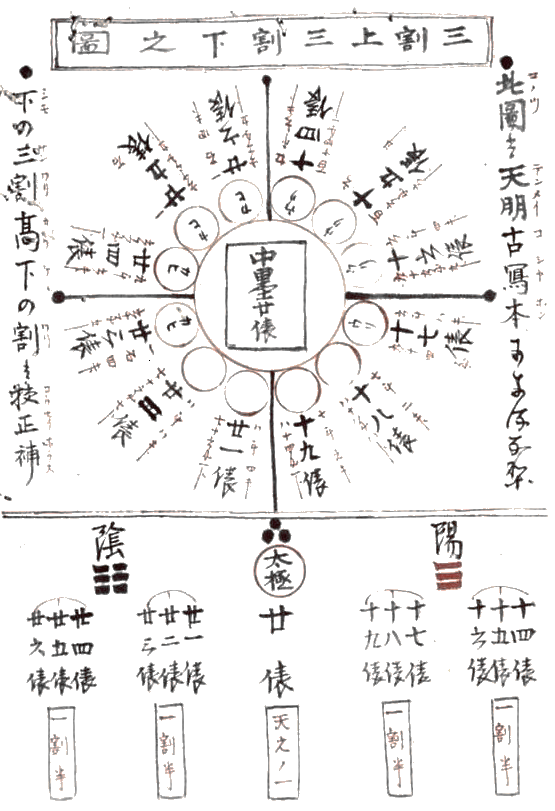
\includegraphics[width=0.85\textwidth]{diagrams/diagram_grand_chart.png}
\caption[The Grand Diagram]{The Grand Diagram (\jp{上割三下割之圖}).
Center: \jp{天明古米} (Tenmei-era old rice) with \jp{中豊横}
(middle-abundance horizontal) as the baseline. Twelve positions radiate
outward representing the months. Bottom left: \jp{陰} (Yin) with
\jp{八極} (Eight Poles)---selling positions at 25, [24], 22, 21 tawara
levels. Bottom right: \jp{陽三} (Yang)---buying positions at 14, [17],
18, 19 tawara levels.\protect\footnotemark{} Bottom annotation:
\jp{平の三割高下の割＝校正補} (``Three-part division of prices, high and
low---revised supplement'').
\textit{Image: Kyoto University Main Library.}}
\label{fig:grandchart}
\vspace*{\fill}
\end{figure}
\footnotetext{Bracketed values [24] and [17] are read directly from
the diagram image but do not appear in the character-by-character
transcription, which records only three values per side (25, 22, 21
and 14, 18, 19). The additional values are legible in the manuscript
but were not captured in the transcription pass.}

\section{How to Read the Diagram}

This diagram, which the source text calls the \jp{中星圓珠秘象}
(``Middle Star Round Jewel Secret Image''), is the visual synthesis of the
entire trading system.\tn{The explanatory text for the diagram spans
manuscript pages 28--29. The diagram's center annotation reads \jp{天明古米}
(\textit{Tenmei-era old rice}), indicating the price data references
the Tenmei period.}

\subsection{Comprehensive Measurement (\jp{度諸})}

\textit{[Interpretive.]}
For 700 ry\=o of capital at various configurations: the positions are
mapped through buying and selling levels, with 300 ry\=o held in
reserve.\tn{The figure \jp{七百両} is tentatively legible. The
surrounding prose is in dense cursive; the rendering here is
interpretive.}

\subsection{The Structure}

The upper half represents the Yang months---spring and summer, the period of
growth and rising. The lower half represents the Yin months---autumn and
winter, harvest and falling. The diagram is oriented like a compass, with
Heaven (\jp{天}) and Earth (\jp{地}) at the poles.

At each month's position: the expected tawara level, the indicated trading
action, and the relationship to the middle star.

The subsidiary charts at the bottom divide the trading range into Yin and
Yang zones. The Yin section (\jp{陰 八極}) maps selling positions at
supply levels of 25, 24, 22, and 21 tawara---representing conditions of
scarcity where prices are high. The Yang section (\jp{陽三}) maps buying
positions at 14, 17, 18, and 19 tawara---representing conditions of
abundance where prices are low.

\subsection{Applying the Diagram}

In the four directions---representing the four seasons---combine the
seasonal tendency with the harvest forecast. When buying in spring, confirm
the middle star, then enter at the ten-percent level.

The rationale for buying and selling at each position is embedded in the
diagram's structure: the monthly tawara level, read against the middle star
and the Yin-Yang subsidiary tables, produces a specific trading action for
any combination of season, supply level, and market momentum.

% =============================================================================
\chapter{Reading Strong and Weak Qi}

\section{The Beginning of Strong Qi}

\textit{[Interpretive.]}
When strong qi first emerges, the signs are these: a rise from the
bottom. People are still bearish. Yet the price has stopped falling and
begins to creep upward.\tn{The header \jp{強氣の初} is legible. The
transcription tentatively identifies \jp{一割} (10\%) and fragments about
sentiment; the connecting prose is interpretive.}

\section{The Beginning of Weak Qi}

\textit{[Interpretive.]}
A small decline from a sustained high. People are still bullish. Yet the
price stops rising and begins to soften.\tn{The header \jp{弱氣の初} is
legible. The prose mirrors the strong qi pattern; both sections are
interpretive reconstructions from partially legible cursive.}

\section{The Great First Decline}

\textit{[Interpretive.]}
The first drop is sharp. But the first major drop is rarely the final
bottom.\tn{The header \jp{大壱落修の事} is legible. The transcription
tentatively identifies fragments about ``the first fall'' being ``sharp''
and ``not the bottom''; the three-phase pattern described here is an
interpretive reconstruction. The pattern---sharp drop, bounce, slow
grind---resembles Dow Theory's description of bear market stages,
formulated roughly fifty years later.}

\section{Wind and Rain}

\textit{[Interpretive.]}
The manuscript discusses \jp{風雨} (wind and rain) and their effect on
the market. A reference to ships (\jp{船}) and storm damage
(\jp{破損}) is legible.\tn{The header \jp{風雨} is legible. The
manuscript mentions months (三月, 四月, 五月, 六月 are legible as
section markers on the left page) with descriptions of seasonal
weather, but the prose between month markers is in dense cursive rated
LOW confidence. The specific agricultural details in previous editions
(frost, plum rains, typhoon timing) were interpretive gap-filling and
have been removed. The characters \jp{油} (oil) and \jp{絹} (silk)
are legible near the bottom of the page.}
The four seasons each bring their own storms, and the trader must
observe them. Oil and silk prices follow similar patterns.

% =============================================================================
\chapter{Regional Markets and Final Teachings}

\section{The Geography of Information}

Each year, the initial rice trading (\jt{初取引}{hatsu-akinai}) establishes
a base price level.\tn{The term \jp{初取引} is legible. \jp{大坂} (Osaka)
and \jp{東國西國} (Eastern and Western Provinces) appear as section
markers. The connecting prose is interpretive, reconstructed from these
anchors and the section's overall theme.}

\textit{[Interpretive.]}
Osaka's D\=ojima exchange is the central rice market; all other regional
prices reference it. Information from Osaka flows outward to the provinces.

Eastern provinces (\jp{東國}) and western provinces (\jp{西國}) have
different harvest cycles.

\section{The World's Accumulation (\jp{世の中積り之事})}

When rice is expensive, all things become dear.\tn{The header
\jp{世の中積り之事} is legible. The phrase \jp{米高きときは万物高し}
(``when rice is high, all things are high'') is tentatively identified
in the transcription. The connecting prose is interpretive.}

\textit{[Interpretive.]}
In all the world's markets, the rice market is the foundation. What has
been written in this record is the accumulated observation of
generations---the secret teachings of the house.

\begin{editorialnote}
The closing pages of the manuscript (pages 31--32) are written in dense
flowing cursive with water damage at the edges. The transcription rates
this section MEDIUM confidence and explicitly warns that it ``cannot
confirm character-by-character'' whether the English corresponds to
specific Japanese sentences. What follows is an interpretive
reconstruction of the afterword's apparent themes. The attribution and
date at the end are clearly legible.
\end{editorialnote}

\textit{[Interpretive.]}
This record should not be shared carelessly. It represents the
accumulated observation of generations.

\begin{flushright}
\jp{鳴川猛之助}\\
\textit{Narukawa Takenosuke}\\
\textit{Editor and Corrector}\\[0.5em]
\jp{嘉永四年五月廿日}\\
\textit{20th day, 5th month, Kaei 4 (1851)}
\end{flushright}

% =============================================================================
\chapter*{Select Bibliography}
\addcontentsline{toc}{chapter}{Select Bibliography}
\markboth{Select Bibliography}{}

\begin{description}[style=nextline, leftmargin=0em, font=\normalfont]

\item CiNii Research. \jp{校正三猿金泉秘録} (\textit{K\=osei Sanen Kinsen
  Hiroku}). Bibliographic record NCID: BD11983527. National Institute of
  Informatics, Japan.
  \url{https://cir.nii.ac.jp/crid/1971712334786825487}

\item Hirschmeier, Johannes, and Tsunehiko Yui. \textit{The Development of
  Japanese Business, 1600--1980}. 2nd ed. London: George Allen \& Unwin,
  1981. ISBN 978-0-04-330322-1.

\item Moss, David A., and Eugene Kintgen. ``The Dojima Rice Market and
  the Origins of Futures Trading.'' Harvard Business School Case 709-044.
  Boston: Harvard Business School Publishing, 2009. Revised 2010.
  \url{https://www.hbs.edu/faculty/Pages/item.aspx?num=36846}

\item Kyoto University Rare Materials Digital Archive. \jp{校正三猿金泉秘録}
  (\textit{K\=osei Sanen Kinsen Hiroku}). Record ID: RB00012360.
  Tanimura Collection, Main Library.
  \url{https://rmda.kulib.kyoto-u.ac.jp/item/rb00012360}

\item National Diet Library, Japan. \jp{校正三猿金泉秘録}. Catalog record.
  Author: \jp{牛田権三郎} (Ushida Gonzabur\=o).
  \url{https://ndlsearch.ndl.go.jp/books/R100000002-I000003283984}

\item Nison, Steve. \textit{Beyond Candlesticks: New Japanese Charting
  Techniques Revealed}. New York: John Wiley \& Sons, 1994.
  ISBN 978-0-471-00720-3.

\item Nison, Steve. \textit{Japanese Candlestick Charting Techniques}.
  2nd ed. New York: Prentice Hall Press, 2001.
  ISBN 978-0-7352-0181-1.

\item Schaede, Ulrike. ``Forwards and Futures in Tokugawa-Period Japan:
  A New Perspective on the D\=ojima Rice Market.'' \textit{Journal of
  Banking \& Finance} 13, no.~4--5 (1989): 487--513.
  DOI: \url{https://doi.org/10.1016/0378-4266(89)90028-9}

\item Takatsuki, Yasuo (\jp{高槻泰郎}). \jp{大坂堂島米市場：江戸幕府vs市場経済}
  (\textit{\=Osaka D\=ojima Kome Shij\=o: Edo Bakufu vs.\ Shij\=o Keizai}).
  Kodansha Gendai Shinsho 2487. Tokyo: Kodansha, 2018.
  ISBN 978-4-06-512498-7.

\item West, Mark D. ``Private Ordering at the World's First Futures
  Exchange.'' \textit{Michigan Law Review} 98, no.~8 (2000): 2574--2615.
  \url{https://repository.law.umich.edu/mlr/vol98/iss8/8/}

\item Zhou Dunyi. \textit{Taijitu shuo} (\jp{太極図説}, Explanation of the
  Diagram of the Supreme Ultimate). Mid-11th century. In Wing-tsit Chan,
  trans.\ and comp., \textit{A Source Book in Chinese Philosophy}, 460--465.
  Princeton: Princeton University Press, 1963.
  ISBN 978-0-691-01964-2.

\end{description}

% =============================================================================
\chapter*{Glossary of Key Terms}
\addcontentsline{toc}{chapter}{Glossary of Key Terms}
\markboth{Glossary of Key Terms}{}

\begin{description}[style=nextline, leftmargin=2em, font=\normalfont\bfseries]

\item[\jp{逢来} (\textit{airai})]
Adverse conditions; a period of generally falling prices, typically lasting
roughly three years within a twelve-to-thirteen-year cycle.

\item[\jp{中星} (\textit{ch\=uboshi})]
Middle Star; the long-term average price level serving as the central
reference for all trading decisions.

\item[\jp{智} (\textit{chi})]
Wisdom; the second of the four trading virtues. Study and observation
before action.

\item[\jp{帳合米} (\textit{ch\=oaimai})]
``Book rice''; forward contracts or futures on rice, as opposed to physical
rice.

\item[\jp{堂島} (\textit{D\=ojima})]
The D\=ojima Rice Exchange in Osaka; the central marketplace for rice
futures trading during the Edo period.

\item[\jp{半板} (\textit{hanita})]
``Half-board''; a method of calculating rice selling positions, as
distinct from the buying-position method.

\item[\jp{穂足} (\textit{hosoku})]
``Spike-foot'' or ``ear of grain''; refers to the visual shape of
price movements---an early form of pattern recognition.

\item[\jp{仁} (\textit{jin})]
Benevolence; the first of the four trading virtues. Patience and
compassion for one's own position and errors.

\item[\jp{人気} (\textit{jinki})]
``People-qi''; market sentiment; the collective mood of traders.

\item[\jp{禁判} (\textit{kinban})]
``Forbidden judgment''; a cautionary ruling or prohibited trading
practice, used as a marker in the Fifteen Articles section.

\item[\jp{順来} (\textit{junrai})]
Favorable conditions; a period of generally rising prices, typically
lasting roughly ten years.

\item[\jp{古米} (\textit{komai})]
Old rice; rice from previous harvests.

\item[\jp{両} (\textit{ry\=o})]
The gold coin unit of the Edo period; the standard unit of capital.

\item[\jp{新米} (\textit{shinmai})]
New rice; freshly harvested rice.

\item[\jp{節} (\textit{setsu})]
Discipline; the fourth of the four trading virtues. Following the method
even when emotions urge otherwise.

\item[\jp{底} (\textit{soko})]
Bottom or floor; the lowest point of the price range.

\item[\jp{底直} (\textit{soko-ne})]
Floor price; the actual price at the lowest point of the range, as
distinct from the abstract concept of ``bottom.''

\item[\jp{太極} (\textit{taikyoku})]
Supreme Ultimate; the Neo-Confucian concept representing undifferentiated
unity, here used for market equilibrium.

\item[\jp{大勢} (\textit{taisei})]
The grand trend; the overarching market direction.

\item[\jp{俵} (\textit{tawara} / \textit{hy\=o})]
A bale of rice; the standard unit of measure and price quotation.

\item[\jp{天井} (\textit{tenj\=o})]
Ceiling; the top of the price range.

\item[\jp{転換の法} (\textit{tenkan no h\=o})]
``Turnover method''; the technique of building selling positions as
buying positions reach their target, revolving from one side of the
market to the other.

\item[\jp{強気} (\textit{tsuyoki})]
Strong qi; bullish sentiment or upward momentum.

\item[\jp{運気} (\textit{unki})]
Fortune-qi; the prevailing momentum of a given period.

\item[\jp{弱気} (\textit{yowaki})]
Weak qi; bearish sentiment or downward momentum.

\item[\jp{勇} (\textit{y\=u})]
Courage; the third of the four trading virtues. Acting decisively when
the signs align.


\item[\jp{随金} (\textit{zuikin})]
``Following gold''; tracking actual capital flows rather than opinion.

\end{description}

% =============================================================================
\chapter*{About the Editor}
\addcontentsline{toc}{chapter}{About the Editor}
\markboth{About the Editor}{}

Zach Booth is a software engineer at NASA Ames Research Center, where
he uses AI systems---including Claude (Anthropic)---in his daily
engineering workflow. Self-taught in Japanese since the age of eighteen
and conversational in the language, he identified this manuscript in
the Kyoto University Rare Materials Digital Archive and recognized that
no accurate English translation existed.

He directed the translation using the same AI tools he works with
professionally, separating transcription from translation, grading each
iteration with an independent reviewer, and publishing the complete
audit trail so that every editorial decision can be checked.

This is his first published translation. The complete source
materials---original manuscript scans, character-by-character
transcription with confidence levels, working translation files, and
\LaTeX{} source---are available at:\\
\url{https://github.com/groverburger/sanen-kinsen-hiroku}

% =============================================================================
\appendix
\chapter{Position Calculation Tables}
\label{app:calctables}

The following sections reproduce the full stage-by-stage position
calculations from the manuscript at each capital level. The source text
presents these as flowing prose with embedded figures, not as formatted
tables---the summary table in \S 7.3.3 is an editorial convenience for
the reader, while this appendix preserves the manuscript's own format.
These are presented as they appear in the source, without editorial
interpolation. See the translator's note in \S 7.3 for an explanation
of the units and methodology.

\section{Trading with 200 Ry\=o (\jp{二百両買})}

\jp{壱}: 200 ry\=o committed. 14 tawara at the middle star.
\jp{一割} (10\%). Position reaches 19 tawara.

\jp{弐}: 100 ry\=o added. 14 tawara per 100 ry\=o. Accumulated
position: 25 tawara at the middle star.

\jp{参}: 100 ry\=o added. Running total: 19 tawara at the middle star.

\jp{四}: Effective exposure: 800 ry\=o. Position squared at a profit,
yielding approximately \jp{六百三拾三俵} (633 tawara) in accumulated
returns.

\section{Trading with 300 Ry\=o (\jp{三百両買})}

\jp{壱}: 300 ry\=o committed. 25 tawara at the middle star.
Strong position (\jp{強氣}). \jp{一割} (10\%).

\jp{弐}: 100 ry\=o added. 18 tawara per entry. Position builds through
the middle star.

\jp{参}: Position compounds. \jp{弐割} (20\%). 17 tawara.

\jp{四}: Capital reaches approximately 800 ry\=o through the staged
method. Middle star level maintained throughout.

\section{Trading with 500 Ry\=o (\jp{五百両買})}

\jp{壱}: 100 ry\=o of the 500 committed initially. 15 tawara.

\jp{弐}: 100 ry\=o added. 14 tawara at the middle star.

\jp{参}: 100 ry\=o added. \jp{弐割} (20\%).

\jp{四}: 14 tawara per stage at the middle star. Position reaches 800+
ry\=o, with positions of approximately 25 tawara.

\section{Scaling to 1,000 Ry\=o (\jp{千両})}

At the 1,000-ry\=o level, the text introduces a five-stage system with
escalating price-movement triggers (\jp{顧氣}---``reflecting on
momentum''):

\jp{壱}: \jp{一割} (10\%). \jp{半年千両} (1,000 ry\=o over half a
year). First entry: 100 ry\=o committed.

\jp{弐}: \jp{二割} (20\%). 100 ry\=o added. Middle star maintained.
14 tawara.

\jp{参}: \jp{二割} (20\%). 300 ry\=o committed. Position accumulates at
the middle star.

\jp{四}: \jp{二割} (20\%). Accumulated position: 14 tawara at full
commitment. Capital noted at approximately 800 ry\=o.

\jp{五}: \jp{三割} (30\%). The final stage---the full cycle is complete.

\vfill

\begin{center}
\rule{2in}{0.4pt}\\[1em]
{\small\itshape End of the Complete Volume}\\[0.3em]
{\small \jp{全} --- \textit{Zen}}
\end{center}

\end{document}
